\section{Self-Supervised Learning: Wav2Vec 2.0}

\begin{frame}{}
    \LARGE \textbf{Self-Supervised Learning: Wav2Vec 2.0}
\end{frame}

\begin{frame}[allowframebreaks]{Wav2Vec 2.0: Overview}
    \begin{figure}
        \centering
        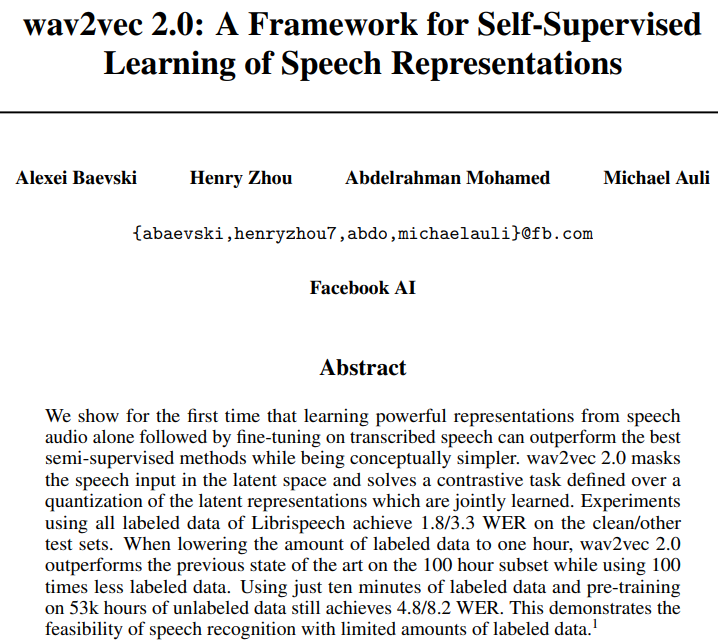
\includegraphics[width=\textwidth,height=0.9\textheight,keepaspectratio]{images/audio-nlp/wav2vec-paper.png}
    \end{figure}
    \begin{itemize}
        \item \textbf{Proposed by Baevski et al. (2020)}
        \item \textbf{Key Idea:} Self-supervised learning for speech representation.
        \item \textbf{Architecture:}
        \begin{itemize}
            \item CNN encoder for raw waveform $\rightarrow$ latent representations $z_t$
            \item Transformer for context representations $c_t$
            \item Quantization module for discrete representations $q_t$
        \end{itemize}
    \end{itemize}
    \begin{figure}[h]
        \centering
        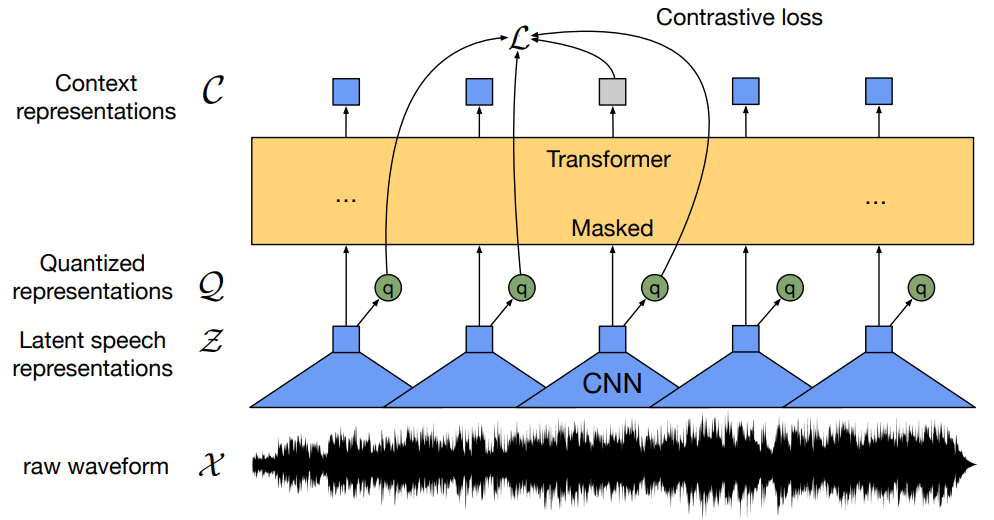
\includegraphics[width=\textwidth,height=0.8\textheight,keepaspectratio]{images/audio-nlp/wav2vec2-overview.png}
        \caption*{Wav2Vec 2.0 architecture overview.}
    \end{figure}
\end{frame}

\begin{frame}{Wav2Vec 2.0: Feature Extraction}
    \begin{itemize}
        \item \textbf{Step 1:} Raw audio waveform is input to a multi-layer CNN encoder.
        \item \textbf{Output:} Latent speech representations $z_t$.
    \end{itemize}
    \begin{center}
        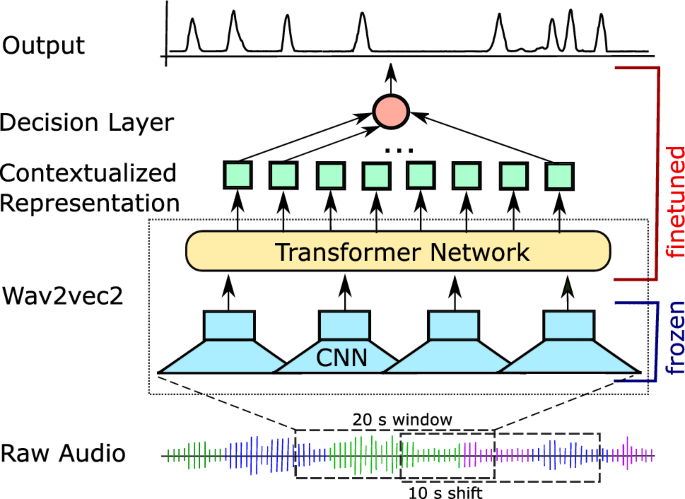
\includegraphics[width=\textwidth,height=0.6\textheight,keepaspectratio]{images/audio-nlp/wav2vec2-cnn.png}
    \end{center}
    \[
        \text{Waveform} \xrightarrow{\text{CNN}} z_t
    \]
\end{frame}

\begin{frame}{Wav2Vec 2.0: Contextualization and Masking}
    \begin{itemize}
        \item \textbf{Step 2:} Random spans of $z_t$ are masked.
        \item \textbf{Step 3:} Transformer network produces contextualized representations $c_t$.
    \end{itemize}
    \[
        z_t \xrightarrow{\text{mask spans}} \xrightarrow{\text{Transformer}} c_t
    \]
\end{frame}

\begin{frame}{Wav2Vec 2.0: Quantization}
    \begin{itemize}
        \item \textbf{Step 4:} Quantize $z_t$ to discrete representations $q_t$.
        \item \textbf{Quantization:} Product of $G$ codebooks, each of size $V$.
    \end{itemize}
    \[
        z_t \xrightarrow{\text{Quantization}} q_t
    \]
\end{frame}

\begin{frame}{Wav2Vec 2.0: Contrastive and Diversity Losses}
    \begin{itemize}
        \item \textbf{Contrastive Loss:} Distinguish true quantized vector $q_t^+$ from negatives $q^-$.
    \end{itemize}
    \[
        L_t = -\log \frac{\exp(\mathrm{sim}(c_t, q_t^+))}{\sum_{q^-} \exp(\mathrm{sim}(c_t, q^-))}
    \]
    \begin{itemize}
        \item \textbf{Diversity Loss:} Encourages usage of all codebook entries.
    \end{itemize}
\end{frame}

\begin{frame}{Wav2Vec 2.0: Performance}
    \begin{itemize}
        \item \textbf{State-of-the-art results:}
        \begin{itemize}
            \item $\sim$1.8\% WER with 960h labeled data
            \item $\sim$4.8\% WER with only 10 minutes labeled data
        \end{itemize}
        \item \textbf{Impact:} Enables efficient use of unlabeled speech data.
    \end{itemize}
    \begin{center}
        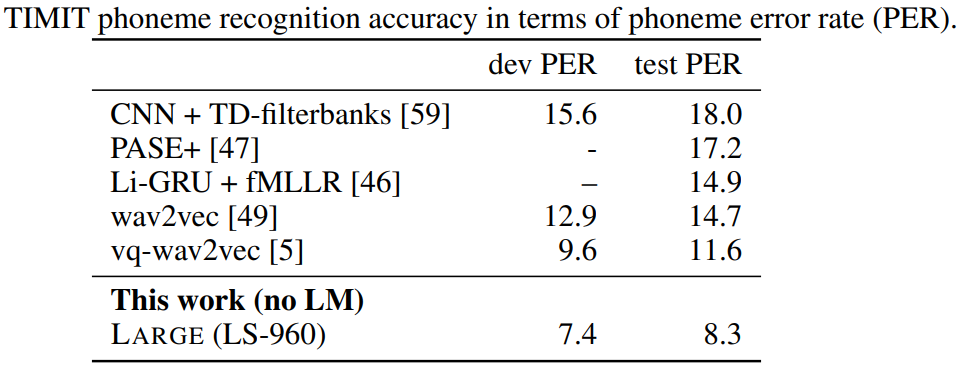
\includegraphics[width=\textwidth]{images/audio-nlp/wav2vec2-results.png}
    \end{center}
\end{frame}